Machine learning is used when the programmer doesn't know all about the domain he is writing for. It is then necessary to have the machine learn by itself by some criteria. Machine learning generally divides into two categories: supervised learning and unsupervised learning. Supervised learning is when you have a known data set where for a known input there will be a known output. In unsupervised learning there is no such data set and the programmer is mostly looking for correlation between the inputs. Unsupervised learning is mostly used for data mining.

Logistic regression is a form of supervised learning which is used for
classification. Our dataset $D$ will consist of the input of the model, a matrix
of the the vectors $\mathbf{x_n}$ and the required outputs $y_n$ for the inputs.
A input vector $\mathbf{x_n}$ will consist of the numerical features of the data
prefixed with a 1 for the bias. $y_n$ can have only 2 values: 1 or -1. There are
more complex forms of logistic regression that can handle more than two values
for $y$ but it is out of the scope of this paper. $N$ will be the size of our
dataset.

\[ D = \{ (\mathbf{x_1}, y_1), (\mathbf{x_2}, y_2), \ldots, (\mathbf{x_N}, y_N)\} \]
\[ \mathbf{x_n} = [ \begin{array}{cccc} 1 & x_1 & \ldots & x_d\end{array} ]^T \]
Similar to another supervised learning algorithm linear regression, logistic
regression is a linear model.``All linear models make use of a "signal" $s$
which is a linear combination of the input vector $\mathbf{x}$ components
weighed by the corresponding components in a weight vector
$\mathbf{w}$.''\cite{website:website:logistic-regression}
\[\mathbf{w} = \left[\begin{array}{cccc} w_0 & w_1 & \ldots & w_d \end{array}
\right]^T \] \[s = w_0 + w_1 x_1 + \cdots + w_d x_d = \sum_{i=0}^d w_i x_i =
\mathbf{w} \cdot \mathbf{x} = \mathbf{w}^T \mathbf{x}\]

Linear regression will use the signal directly as output, but logistic
regression will pass the signal through a sigmoid or logistic function and treat
thats output as the probability that $y=1$.

\[h(\mathbf{x}) = \theta(s)\]
\[\theta(s) = \frac{e^s}{1+e^s} = \frac{1}{1 + e^{-s}}\]

%\usepackage{graphics} is needed for \includegraphics
\begin{figure}[htp]
\begin{center}
  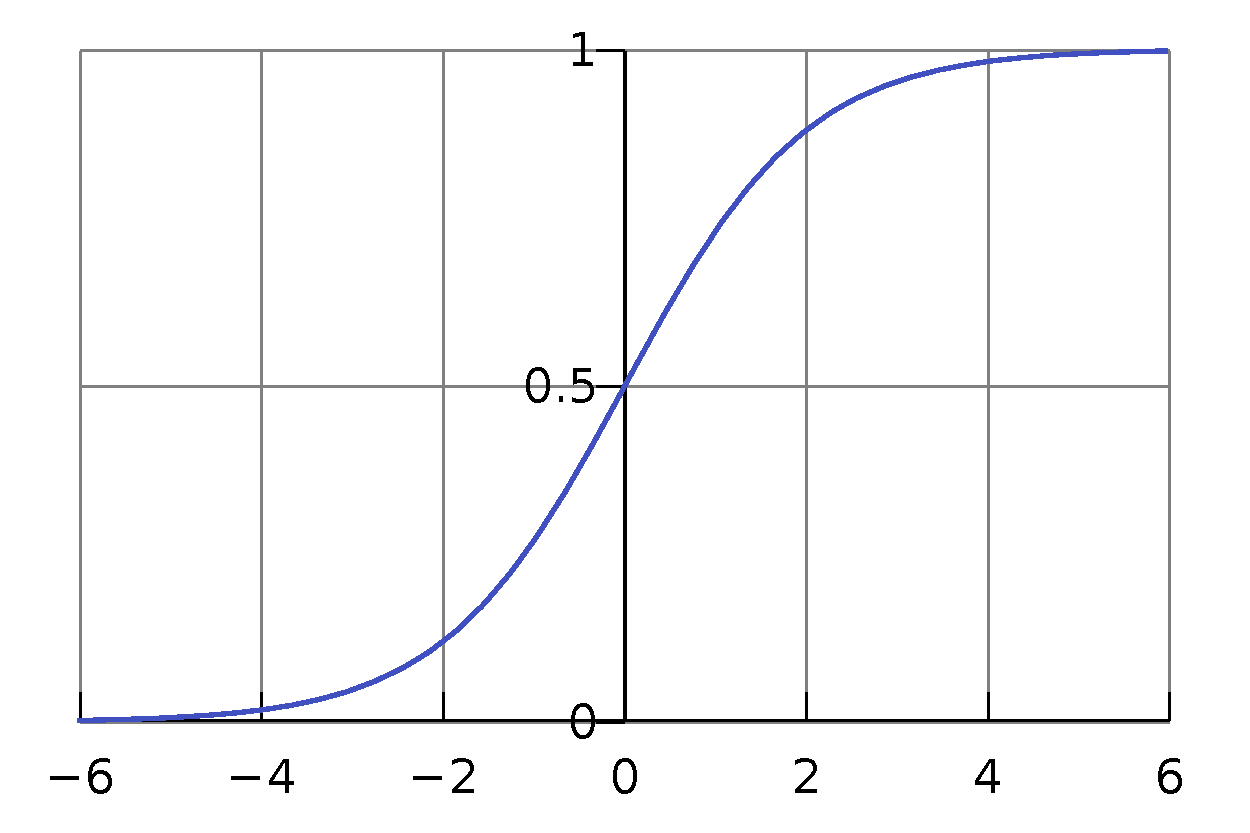
\includegraphics[width=\textwidth]{logistics-curve}
  \caption[Logistics curve]{The shape of a logistics curve.}
  \label{logistics-curve}
\end{center}
\end{figure}

As shown in figure \ref{logistics-curve}, the logistic function is good for
translating between linear values and probability, because the higher the linear value, the higher the probability of the output value being 1 and the lower the linear value the higher the probability of the output being -1. At input value 0, the probability of it being either value is 0.5.

``We say that the data is generated by a noisy
target.''\cite{website:logistic-regression} \[ P(y|\mathbf{x}) = \left\{
\begin{array}{ll}
f(\mathbf{x}) & \mbox{for } y = +1 \\
1 - f(\mathbf{x}) & \mbox{for } y = -1
\end{array} \right. \]
We want to learn a hypothesis $h(x)$ that best fits the above target according to some error function.
\[h(\mathbf{x}) = \theta \left( \mathbf{w}^T \mathbf{x} \right)\approx f(\mathbf{x})\]
``It's important to note that the data does not tell you the probability of a
label but rather what label the sample has after being generated by the target
distribution.''\cite{website:logistic-regression}. The goal of the training will be to calculate the weight vector w so that it minimizes some kind of in-sample error measure.
\[\mathbf{w}_h = \argmin_w E_{in} (\mathbf{w})\]

Our error measure will be based on likelihood. Likelihood is the probability of
generating the data with a model. Likelihood will be high if the hypothesis is
similar to the target distribution. Let's assume that the data was generated by
the hypothesis:

\[P(y|\mathbf{x}) = \left\{ 
\begin{array}{ll}
h(\mathbf{x}) & \mbox{for } y = + 1 \\
1 - h(\mathbf{x}) & \mbox{for } y = -1
\end{array}
\right.\]
\[h(\mathbf{x}) = \theta (\mathbf{w}^T \mathbf{x})\]

Let's try to remove the cases using the property $\theta(-s) = 1 - \theta (s)$.
\[\left.
\begin{array}{l}
\mbox{if $y=+1$ then } h(\mathbf{x}) = \theta (\mathbf{w}^T \mathbf{x}) = \theta (y \mathbf{w}^T \mathbf{x}) \\
\mbox{if $y=-1$ then } 1 - h(\mathbf{x}) = 1 - \theta (\mathbf{w}^T \mathbf{x}) = \theta (-\mathbf{w}^T \mathbf{x}) = \theta (y \mathbf{w}^T \mathbf{x})
\end{array}
\right\} P(y | \mathbf{x}) = \theta(y \mathbf{w}^T \mathbf{x})\]
Let's denote an arbitrary hypothesis g, in which case the likelyhood is defined as:
\[L(D|g) = \prod_{n=1}^N P(y_n | \mathbf{x}_n) = \prod_{n=1}^N \theta(y_n \mathbf{w}_g^T \mathbf{x}_n)\]
To find the best hypothesis, we have to find the best weight vector $\mathbf{w}$.
\begin{eqnarray*}
\mathbf{w} & = & \argmax_\mathbf{w} L \left( D|h \right) = \argmax_\mathbf{w} \prod_{n=1}^N  \theta \left( y_n \mathbf{w}^T \mathbf{x}_n \right) = \argmax_\mathbf{w} \ln \left( \prod_{n=1}^N \theta\left( y_n \mathbf{w}^T \mathbf{x}_n \right) \right) \\
& = & \argmax_\mathbf{w} \frac{1}{N} \ln \left( \prod_{n=1}^N \theta \left( y_n \mathbf{w}^T \mathbf{x}_n \right) \right) = \argmin_\mathbf{w} \left[ - \frac{1}{N} \ln \left( \prod_{n=1}^N \theta \left( y_n \mathbf{w}^T \mathbf{x} \right) \right) \right] \\
& = & \argmin_\mathbf{w} \frac{1}{N} \sum_{n=1}^N \ln \left( \frac{1}{\theta \left( y_n \mathbf{w}^T \mathbf{x}_n \right)} \right) = \argmin_\mathbf{w} \frac{1}{N} \sum_{n=1}^N \ln \left( 1 + e^{-y_n \mathbf{w}^T \mathbf{x}_n} \right)
\end{eqnarray*}
We have derived a good form for the error measure, which is the loss function or the average point error.
\[ E_{in} \left( \mathbf{w} \right) = \frac{1}{N} \sum_{n=1}^N \ln \left( 1 + e^{-y_n \mathbf{x}_n \mathbf{w}^T} \right) = \frac{1}{N} \sum_{n=1}^N e \left( h \left( \mathbf{x}_n \right), y_n \right) \]
\[ e \left( h \left( \mathbf{x}_n \right), y_n \right) = \ln \left( 1 + e^{-y_n \mathbf{x}_n \mathbf{w}^T} \right) \]
We minimise the error function using gradient descent. Gradient descent works by moving the current value towards the local minimum. With the derivative, one can calculate the necessary direction and the rough distance of the local minimum from the current value. Therefore training works with the formula:
\[ \mathbf{w}_{i+1} = \mathbf{w}_i - \eta \nabla E_{in} \left( \mathbf{w}_i \right) \]
Where $\eta$ is the learning rate. We need the derivative of the point error function and the average point error.
\[ \frac{d}{d \mathbf{w}} e \left( h \left( \mathbf{x}_n \right), y_n \right) = \frac{-y_n \mathbf{x}_n e^{-y_n \mathbf{w}^T \mathbf{x}_n}}{1 + e^{-y_n \mathbf{w}^T \mathbf{x}_n}} = -\frac{y_n \mathbf{x}_n}{1 + e^{y_n \mathbf{w}^T \mathbf{x}_n}} \]
\begin{eqnarray*}
\nabla E_{in} \left( \mathbf{w} \right) & = & \frac{d}{d \mathbf{w}} \left[ \frac{1}{N} \sum_{n=1}^N e \left( h \left( \mathbf{x}_n \right), y_n \right) \right] = \frac{1}{N} \sum_{n=1}^N \frac{d}{d \mathbf{w}} e \left( h \left( \mathbf{x}_n \right), y_n \right) \\
& = & \frac{1}{N} \sum_{n=1}^N \left( -\frac{y_n \mathbf{x}_n}{1 + e^{y_n \mathbf{w}^T \mathbf{x}_n}} \right) = - \frac{1}{N} \sum_{n=1}^N \frac{y_n \mathbf{x}_n}{1 + e^{y_n \mathbf{w}^T \mathbf{x}_n}}
\end{eqnarray*}
\[ \mathbf{w}_{i+1} = \mathbf{w}_i - \eta \left( -\frac{1}{N} \sum_{n=1}^N \frac{y_n \mathbf{x}_n}{1 + e^{y_n \mathbf{w}_i^T \mathbf{x}_n}} \right) = \mathbf{w}_i + \eta \left( \frac{1}{N} \sum_{n=1}^N \frac{y_n \mathbf{x}_n}{1 + e^{y_n \mathbf{w}_i^T \mathbf{x}_n}} \right) \]
To lower the number of iterations, each feature of $\mathbf{x}$ should be
normalised before it is used for predicting or training the model. Normalising
means that the program calculates the standard score of each of the features
which is then used instead. The standard score subtracts the mean from the
features and divides that with the standard deviation of the values. A values
standard score floats around the 0 value and roughly has the same absolute value
as other standard scores. When normalising $\mathbf{x}$ for predicting, the mean
and standard deviation cannot be enhanced with that data, because then the
trained model will not be expecting such data. It would mean comparing two
fundamentally different sets of data. It is important to note that the bias
variable in $\mathbf{x}$ should not be normalised, because it will end in a
divide by zero error.\cite{website:normalisation}
